%
%  $Description: Author guidelines and sample document in LaTeX 2.09$
%
%  $Author: ienne $
%  $Date: 1995/09/15 15:20:59 $
%  $Revision: 1.4 $
%

\documentclass[times, 10pt,twocolumn]{article}
\usepackage[brazil]{babel}
\usepackage[utf8]{inputenc}
\usepackage[T1]{fontenc}
\usepackage{latex12}
\usepackage{times}
\usepackage{balance}
\usepackage{graphicx}
\usepackage{amsfonts,amssymb}
\usepackage{subfigure}
%\usepackage{multirow,multicol} %trabalhar com tabelas

%\documentstyle[times,art10,twocolumn,latex8]{article}

%-------------------------------------------------------------------------
% take the % away on next line to produce the final camera-ready version
\pagestyle{empty}

%-------------------------------------------------------------------------
\begin{document}



\title{Aplicação de análise morfológica para \\segmentação de páginas em imagens de documentos}
\author{Aluno: Ricardo de Cillo\\
%\emph{Universidade Estadual de Santa Cruz}\\
%\emph{and University of S\~ao Paulo, Brazil}\\
%\emph{mmbertoldi@uesc.br}\\
% For a paper whose authors are all at the same institution,
% omit the following lines up until the closing ``}''.
% Additional authors and addresses can be added with ``\and'',
% just like the second author.
\and
Supervisora: Nina S. T. Hirata \\
%\emph{Dept. of Computer Science}\\
%\emph{Institute of Mathematics and Statistics}\\
%\emph{University of S\~ao Paulo, Brazil}\\
%First line of institution2 address\\ Second line of institution2 address\\
%\emph{nina@ime.usp.br}\\
}

\maketitle
\thispagestyle{empty}



\section{Introdução}

Uma das aplicações da teoria de visão computacional é a análise de
imagens de documentos. A análise de imagens de documentos, ou apenas
análise de documentos, é um campo de pesquisa atualmente ainda
bastante ativo apesar de estar sendo explorado desde algumas décadas
atrás~\cite{10.1109/ICDAR.2007.207}. Isto se deve a sua importância
prática e a complexidade dos problemas abordados.

O diagrama \ref{fig:context1}, adaptado de
\cite{Kasturi_OGorman_Govindaraju_2002}, mostra os diferentes
problemas abordados nesse campo de pesquisa. 

\begin{figure*}[htb!]
\begin{center}
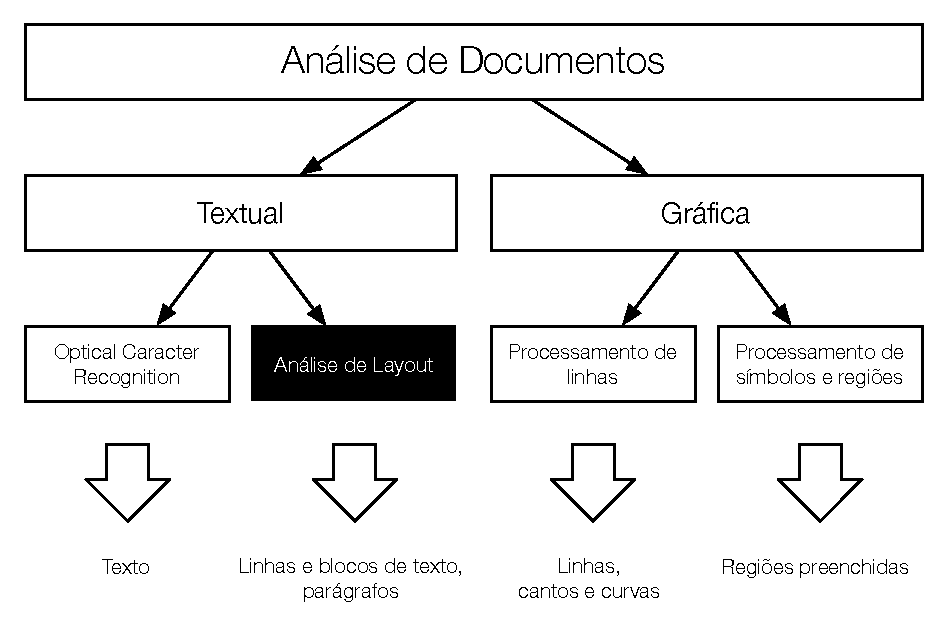
\includegraphics[width=0.8\textwidth]{assets/document_processing_areas_hierarquies.pdf}
\end{center}
\caption{Contextualização do tema do trabalho entre as áreas da análise de documentos.}
\label{fig:context1}
\end{figure*}

Em análise de documentos, o objetivo é extrair informações sobre o
conteúdo e estrutura de um documento digitalizado. Uma das etapas
envolvidas nesse processo é a segmentação de página que consiste na
identificação de áreas da imagem correspondentes à elementos
estruturais, tais como títulos, legendas e blocos de texto.
(é isso que é chamado de análise de alyout?)

Diferentes técnicas de processamento e análise de imagens têm sido
propostos e aplicados na segmentação de páginas.

O objetivo deste trabalho é investigar algumas das técnicas usadas
para segmentação de páginas e explorar a aplicação de operadores
morfológicos~\cite{Serra:1983:IAM:1098652} à segmentação de páginas. A qualidade da solução
obtida será medida e comparada, segundo os mesmo critérios aplicados à
resultados considerados estado da arte por pesquisadores da área
\cite{10.1109/ICDAR.2007.207}.


\section{Metodologia}

Uma grande diversidade de métodos já foram explorados na solução do
problema de segmentação de
páginas. Em~\cite{Antonacopoulos95representationand} os autores
propõem um método
que observa a distribuição dos espaços em branco em um documento para
classificar a região em texto ou não. Já
em~\cite{Moll07documentcontent} extrai-se características dos pixels e
sua vizinhança, classificando-os e depois agrupando-os em regiões.


\subsection{Treinamento de operadores morfológicos}

Os operadores morfológicos~\cite{Serra:1983:IAM:1098652} são bastante
utilizados na área de visão computacional, para diferentes tipos de
processamento de imagens. A construção de operadores morfológicos
eficazes consiste em geral na combinação sequencial de operadores
simples e pode ser uma tarefa difícil, além de demandar muita
experiência. Portanto, neste trabalho propomos a construção de tais
operadores, para a tarefa de segmentação de páginas, de forma
automática a partir de imagens de treinamento, como descrito em
\cite{Tomita:1996:PrAuMa}.

A figura~\ref{fig:schema_overview} ilustra o esquema geral de
construção de um operador morfológico baseado em treinamento.
\begin{figure*}[htb!]
\begin{center}
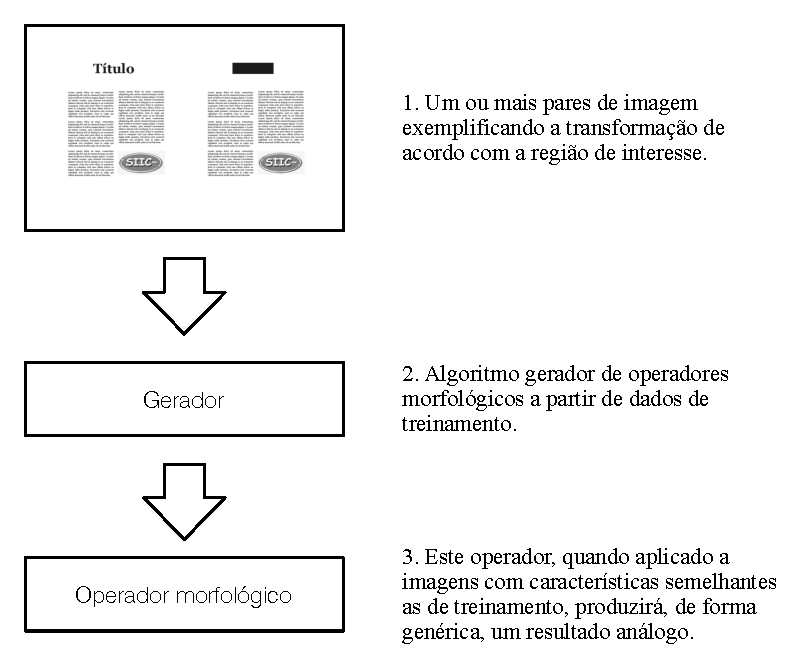
\includegraphics{assets/methodology.pdf}
\end{center}
\caption{Visão global do funcionamento.}
\label{fig:schema_overview}
\end{figure*}

As imagens binárias definidas em um certo domínio $E$ (geralmente
$E=\mathbb{Z}^2$) podem ser modeladas por uma função $f: E \to
\{0,1\}$ tal que $f(x)=1$ se e seomente se $x$ é um pixel
correspondente a um objeto na imagem (portanto, $f(x)=0$ se $x$
é um pixel do fundo (\emph{background}) da imagem).

O conjunto de todas as imagens binárias definidas em $E$ é denotado
por $\{0,1\}^E$. Desta forma, um operador de imagens binárias é um
mapeamento do tipo $\Psi: \{0,1\}^E \to \{0,1\}^E$. 

Seja $W$ uma janela de observação. Imagens podem ser processadas pixel
a pixel, considerando-se a vizinhança de cada pixel definida pela
janela $W$. Tais processaemntos podem ser caracterizados por uma
função do tipo $\psi: \{0,1\}^W \to \{0,1\}$, da seguinte forma
\begin{equation}
[\Psi(f)](x) = \psi(f_{-x}|_W)
\end{equation} 
na qual $f_{-x}|_W$ representa a imagem binária $f$ restrita a $W$ em
torno de $x$.

O erro de um operador é caracterizado por
\begin{equation}
MAE\langle \Psi \rangle = E \big[ [\Psi(S)](z) - I(z) \big]\,.
\end{equation}
Supondo estacionaridade, o ponto $z$ é arbitrário. Na prática o erro é
calculado tomando-se a média do erro absoluto computado sobre
todos os pixels da imagem.

Portanto, o problema de projetar operadores morfológicos localmente
caracterizados reduz-se ao problema de projetar funçõs binárias do
tipo $\psi: \{0,1\}^W \to \{0,1\}$.
Dado que $P$ é a distribuição conjunta do processo
$(\mathbf{X},\mathbf{y})$ (padrões observados pela janela $W$ e
respectivo valor da imagem de saída para o pixel considerado), pode-se
mostrar que o operador ótimo em relação ao erro MAE é dado por
\begin{equation}
\label{eq:opt}
\psi(X) = \left\{
          \begin{array}{ll}
          1, & \mbox{se $P(X,0)<P(X,1)$,}\\
          0, & \mbox{se $P(X,0)>P(X,1)$,}\\
          1 \mbox{ ou } 0, & \mbox{if $P(X,0)=P(X,1)$.}
          \end{array}
\right.
\end{equation}

Na prática, essas probabilidades não são conhecidas. Portanto, no
processo de aprendizado de operadores as mesmas são estimadas a partir
de imagens de treinamento (pares de imagens entrada-saída, sendo que
as imagens de saída em geral são geradas editando-se a imagem de
entrada). A partir das probabilidades estimadas, pode-se obter a
decisão ótima de acordo com a equação~\ref{eq:opt}. No entanto, nem
todos os padrões $X$ são observados nas imagens de
treinamento. Portanto, utiliza-se um algoritmo de aprendizado para que
a função característica do operador resultante fique completamente
definida. Frequentemente, a esse processo de atribuir uma
classificação para os padrões não pertencentes ao conjunto de
treinamento é denominado de generalização.

Diferentes algoritmos de aprendizado podem ser
utilizados. Em~\cite{Tomita:1996:PrAuMa} utiliza-se a minimização de
funções booleanas não especificadas completamente.


\subsection{Avaliação da segmentação}

O desempenho de algoritmos de processamento de imagens pode ser
avaliado comparando-se os resultados gerados pelo algoritmo com os
resultados esperados. Para uma avaliação objetiva, métricas de
comparação podem ser usadas. Neste trabalho usamos tal tal métrica.

Descrever a tal tal métrica.


\section{Resultados esperados}

Alguns resultados publicados atestam a viabilidade dessa abordagem
(citar artigo do sibgrapi). No entanto, nesses trabalhos a segmentação
de páginas é apresentada apenas como um exemplo de possível aplicação,
não tendo sido o alvo de investigação.

Os experimentos serão realizados com  diferentes conjuntos de dados, a
saber:

\begin{itemize}
\item X
\item Y
\end{itemize}

Para o treinamento do operador morfológico será utilizado o pacote
TRIOS, ..... (descrever o pacote).

Finalmente, os resultados obtidos serão comparados com os resultados
esperados (\emph{ground-truth}), segundo a métrica descrita acima.


{\small 
\bibliographystyle{plain}	% (uses file "plain.bst")
\bibliography{myrefs}		% expects file "myrefs.bib"
}

\end{document}

